\documentclass[11pt,letterpaper,spanish]{article}

\usepackage{bbm}
\usepackage{amsmath, amsthm, amssymb}
\usepackage{geometry} % to change the page dimensions
\geometry{letterpaper} % or letterpaper (US) or a5paper or....

%PAquetes
\usepackage{babel}
\usepackage{graphicx}
\usepackage[utf8]{inputenc}
\pagestyle{myheadings}
\usepackage{verbatim}  
\usepackage{enumerate}
\usepackage{subfig}
\usepackage{fancyhdr} 
\pagestyle{fancy} 
\usepackage{multicol}
\usepackage{rotating}
\usepackage{bbm}
\usepackage{float}
\usepackage{amsmath, amsthm, amssymb}
\usepackage{setspace}
\usepackage{titlesec} 
\usepackage{marvosym}
\usepackage{hyperref}

\usepackage{svg}

\lhead{}\chead{}\rhead{}
\lfoot{}\cfoot{}\rfoot{}

\renewcommand{\headrulewidth}{0.1pt} 
\renewcommand{\footrulewidth}{0.1pt}
\pagenumbering{arabic}

\setlength{\parindent}{0cm}

\fancyhead[R]{\small \scshape Carlos Petricioli}
\fancyhead[C]{\small \color{blue}  \href{http://carlospetricioli.com}{carlospetricioli.com} }
\fancyhead[L]{\small \scshape Proyecto visualización UCSD}
\fancyfoot[L]{\small Fecha: \today.}
\fancyfoot[R]{\small  Página \thepage \ de \pageref{LastPage}}


\titleformat{\section}{\scshape \centering \Large}{}{0em}{}[] 

\setstretch{1.15}
 


\usepackage{tabularx,colortbl} % Advanced table configurations
%\usepackage{fontspec} % Allows font customization
\usepackage{color}

\usepackage{xcolor,colortbl}



\begin{document}
\section{Propuesta para ``Proyecto  de visualización UCSD''\\ }
\subsection*{Descripción}

El objetivo del proyecto es hacer una visualización para un atlas de salud en México.
Módulos a desarrollar:
\begin{enumerate}
\item MHD–DataBook: Sistema para consultar la base de datos del proyecto.
\item Fact Sheets: Fichas por estado y municipio que presenten información
homologada ya seleccionada.
\item Herramienta de Análisis: Sistema que permita realizar comparativos entre
estados y municipios con base en las principales categorías de información y datos.
\end{enumerate}

Para atender estos módulos se sugieren visualizaciones como las siguientes (\href{http://carlospetricioli.com/propuesta_sigmum}{\color{blue}link}):


\begin{figure}[H]
\caption{Círculos}
\centering
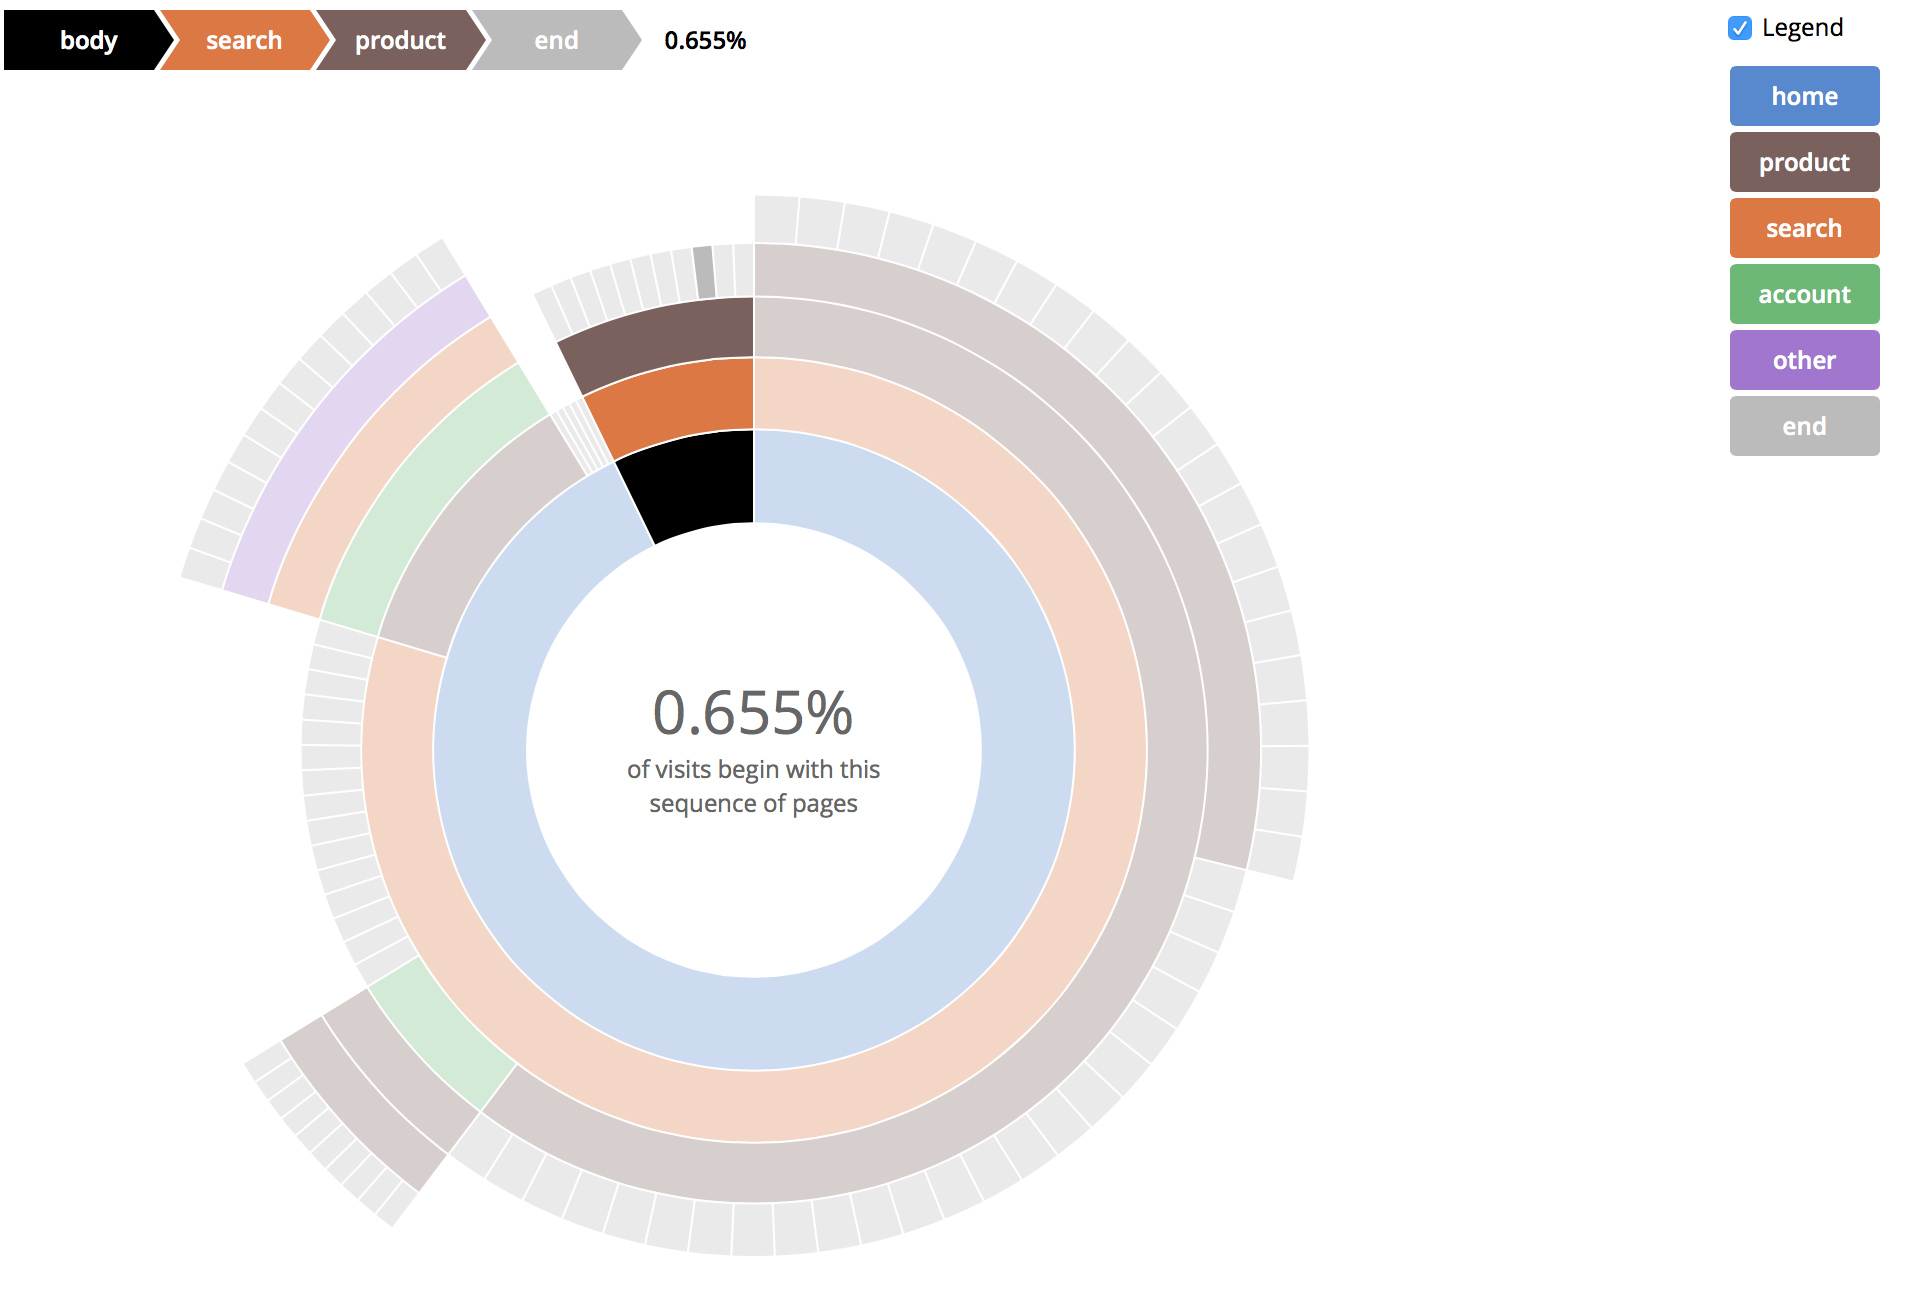
\includegraphics[width=110mm]{../img/circulos.png}
\end{figure}

\begin{figure}[H]
\caption{Filtros}
\centering
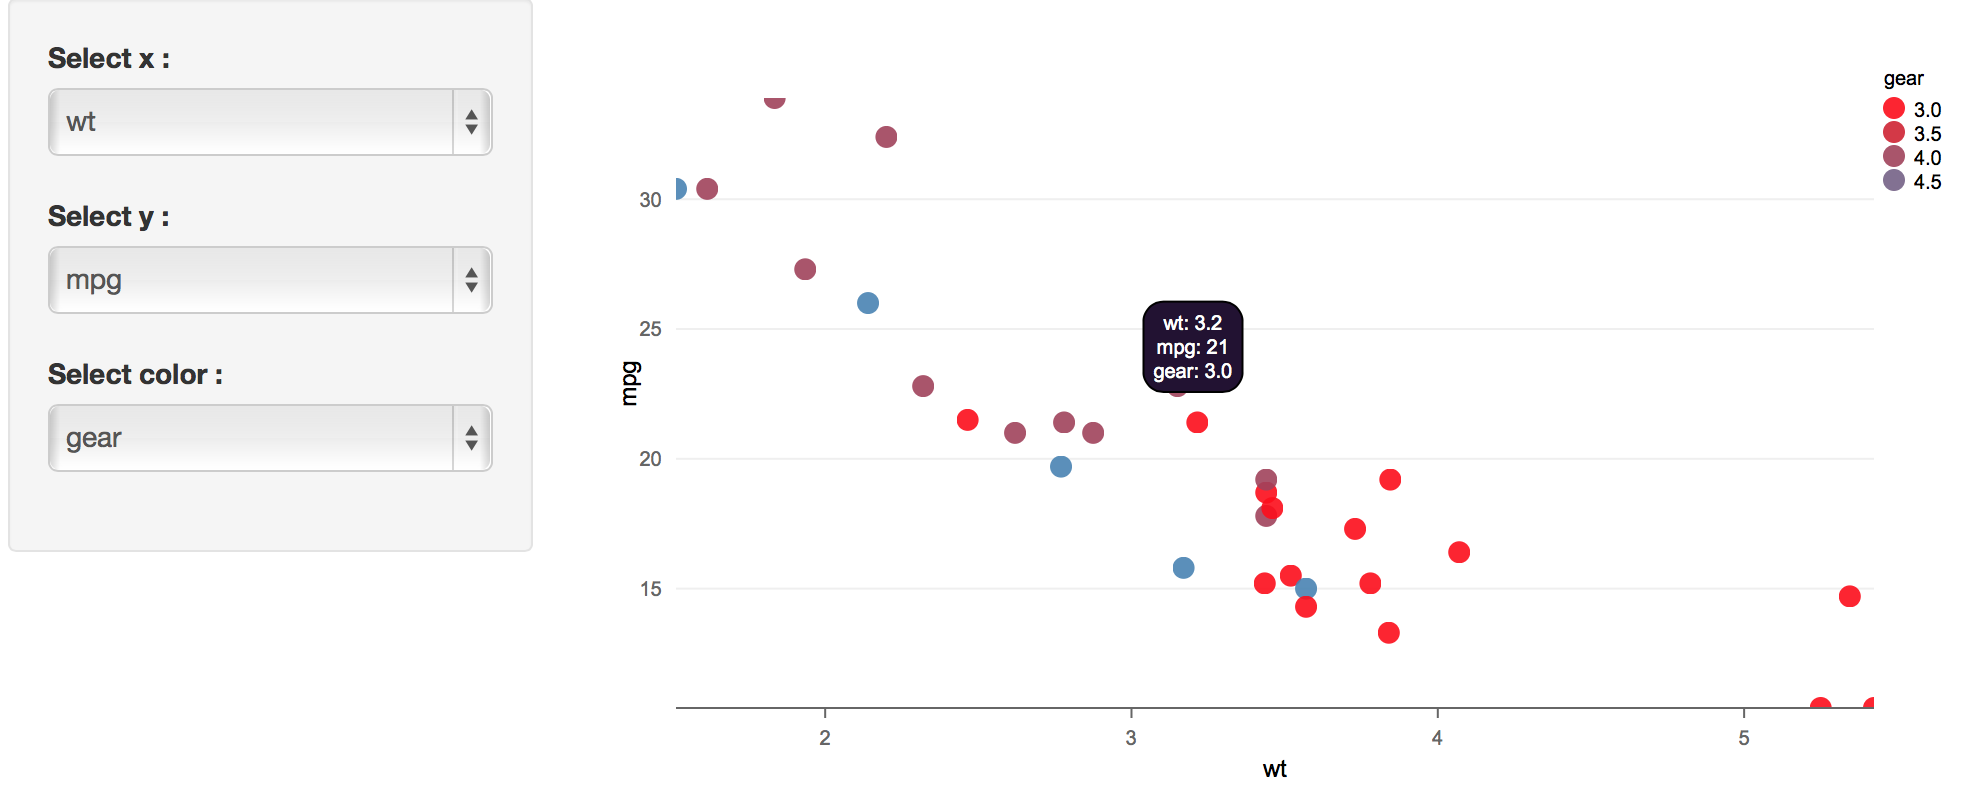
\includegraphics[width=150mm]{../img/filtros.png}
\end{figure}

\begin{figure}[H]
\caption{Gráfica de pirámide}
\centering
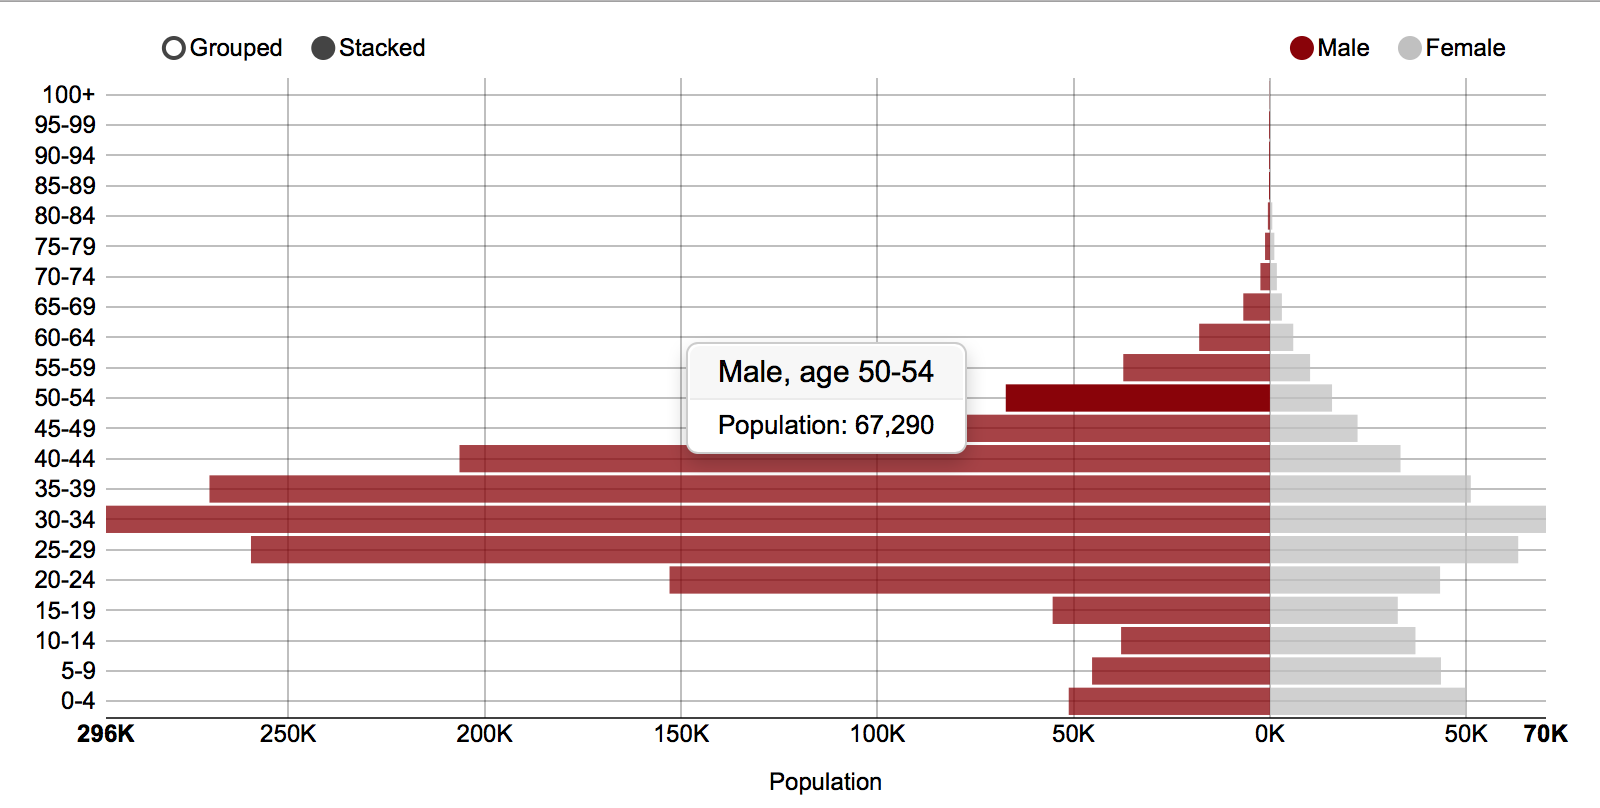
\includegraphics[width=150mm]{../img/piramide.png}
\end{figure}

\begin{figure}[H]
\caption{Animación de burbujas}
\centering
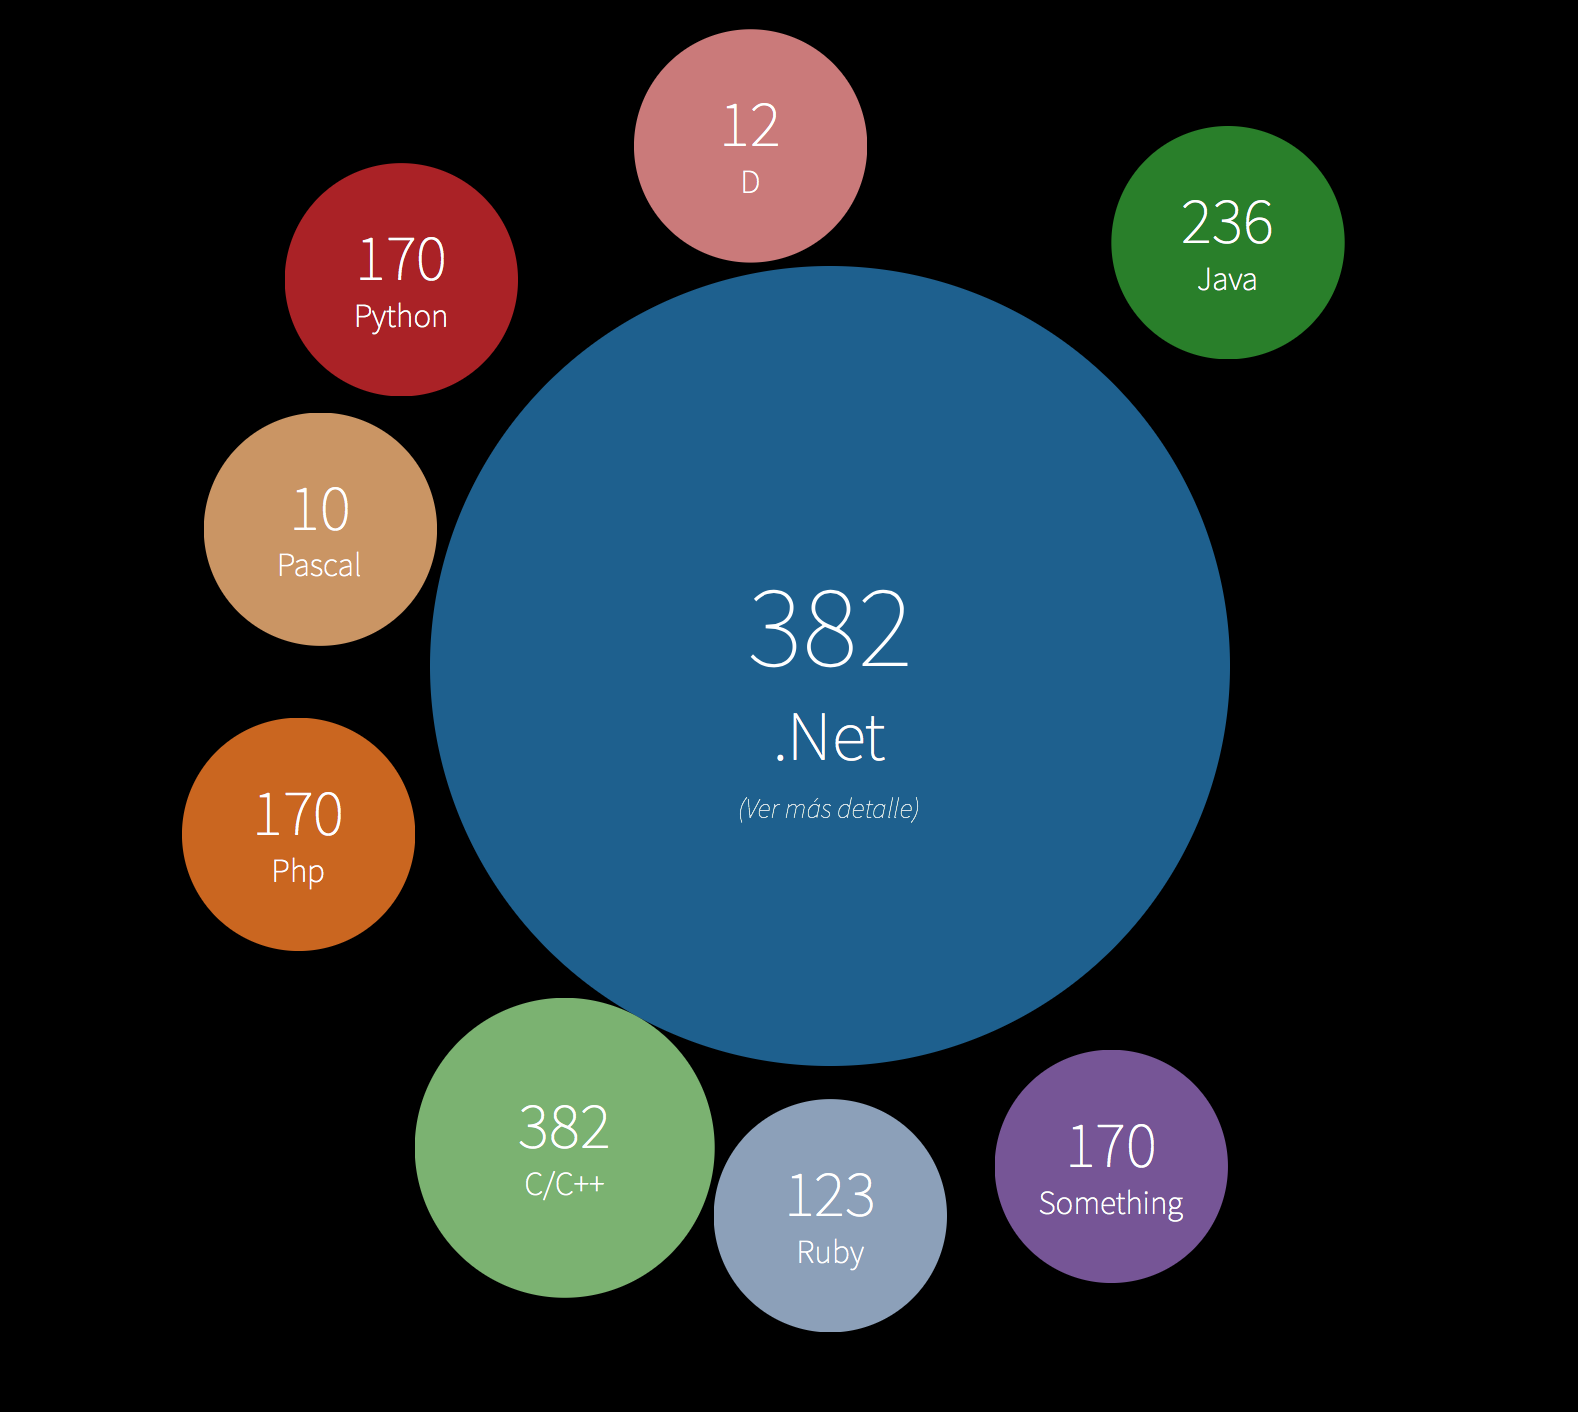
\includegraphics[width=90mm]{../img/burbujas.png}
\end{figure}

\newpage

\subsection*{Estimado de tiempo}

La fecha propuesta para el inicio del proyecto es el \texttt{lunes 5 de enero del 2015} y tendrá fecha de entrega final el \texttt{27 de febrero del 2015}. El tiempo aproximado que tendrá cada parte del proyecto se detalla a continuación.



\begin{table}[H]
\caption{Tabla de tiempos estimados}
\centering
\begin{tabular}{lr}
\hline
& Tiempo requerido \\
Descripción & (días habiles)\\
\hline
1. Entrega de los datos y familiarización & 5\\
2. Diseño de visualización & 10\\
3. Implementación de la visualización & 20\\
4. Pruebas e instalación del entregable  & 5 \\
\hline
Total & 40\\
\hline
\end{tabular}
\end{table}


\subsection*{Personas involucradas en el proyecto y en qué capacidad actúan}

Carlos Petricioli como líder del proyecto y un asesor personal por definir más adelante. 

\subsection*{Estimado de recursos que se requieren}

Se solicita una cantidad de MXN\$\textit{130,000.00} (ciento treinta mil pesos) más el correspondiente  impuesto al valor agregado, misma que se pagará al finalizar el proyecto. Se requiere un anticipo del 30\% de dicho monto a ser pagado el día de inicio del proyecto.

\label{LastPage}
\end{document}